\documentclass[11pt,a4paper]{article}

% ============================================================
% PAQUETES BÁSICOS
% ============================================================
\usepackage{fontspec}
\setmainfont{Myriad Pro}    % Fuente principal
\usepackage[spanish]{babel}
\usepackage{graphicx}
\usepackage{geometry}
\usepackage{fancyhdr}
\usepackage{titlesec}
\usepackage{xcolor}
\usepackage{hyperref}
\usepackage{amsmath}        % Para ecuaciones matemáticas
\usepackage{float}          % Para mejor control de posición de figuras
\usepackage{caption}        % Para personalizar captions
\usepackage{subcaption}     % Para subfiguras si se necesitan
\usepackage{microtype}      % Mejora el espaciado y reduce overfull
\usepackage{eso-pic}        % Paquete clave para añadir imágenes de fondo
% Paquetes recomendados para tablas
\usepackage{placeins}       % \FloatBarrier para controlar floats
\usepackage{booktabs}       % Reglas profesionales (\toprule, \midrule, \bottomrule)
\usepackage{tabularx}       % Columnas X que ajustan al ancho
\usepackage{array}          % Control avanzado de columnas
\newcolumntype{L}{>{\raggedright\arraybackslash}X} % Columna X alineada a la izquierda


% ============================================================
% CONFIGURACIONES BÁSICAS
% ============================================================

% Configuración de márgenes
\geometry{
    top=2.5cm,
    bottom=2.5cm,
    left=2cm,
    right=2cm,
    headheight=14.5pt
}

% Configuración de enlaces
\hypersetup{
    colorlinks=true,
    linkcolor=blue,
    filecolor=magenta,
    urlcolor=cyan,
    pdftitle={Memoria Práctica},
    pdfpagemode=FullScreen,
}

% Configuración de encabezados y pies de página
\pagestyle{fancy}
\fancyhf{}
\fancyhead[L]{Asignatura - Nº Práctica}
\fancyhead[R]{Mes - Año}
\fancyfoot[R]{\thepage}
\fancyfoot[L]{Nombre del Estudiante}

% ============================================================
% CONFIGURACIONES ESPECÍFICAS POR ASIGNATURA
% ============================================================

% --- [SISTEMAS OPERATIVOS] Configuración de listings para código ---
\usepackage{listings}

% Configuración de colores para el código
\definecolor{codegreen}{rgb}{0,0.6,0}
\definecolor{codegray}{rgb}{0.5,0.5,0.5}
\definecolor{codepurple}{rgb}{0.58,0,0.82}
\definecolor{backcolour}{rgb}{0.95,0.95,0.92}
\definecolor{codeorange}{rgb}{0.8,0.4,0}
\definecolor{framecolor}{rgb}{0.7,0.7,0.7}

% Configuración de listings para código C
\lstdefinestyle{mystyle}{
    backgroundcolor=\color{backcolour},   
    commentstyle=\color{codegreen}\itshape,
    keywordstyle=\color{blue}\bfseries,
    numberstyle=\tiny\color{codegray},
    stringstyle=\color{codepurple},
    basicstyle=\ttfamily\small,
    breakatwhitespace=false,         
    breaklines=true,                 
    captionpos=b,                    
    keepspaces=true,                 
    numbers=left,                    
    numbersep=8pt,
    showspaces=false,                
    showstringspaces=false,
    showtabs=false,                  
    tabsize=4,
    frame=single,
    frameround=tttt,
    rulecolor=\color{framecolor},
    framesep=4pt,
    xleftmargin=15pt,
    xrightmargin=5pt,
    language=C,
    extendedchars=true,
    inputencoding=utf8,
    escapeinside={(*@}{@*)},
    morecomment=[l][\color{codeorange}]{\#},
    columns=flexible,
    aboveskip=15pt,
    belowskip=10pt,
    literate={á}{{\'a}}1 {é}{{\'e}}1 {í}{{\'i}}1 {ó}{{\'o}}1 {ú}{{\'u}}1
             {Á}{{\'A}}1 {É}{{\'E}}1 {Í}{{\'I}}1 {Ó}{{\'O}}1 {Ú}{{\'U}}1
             {ñ}{{\~n}}1 {Ñ}{{\~N}}1 {¿}{{?`}}1 {¡}{{!`}}1
}

\lstset{style=mystyle}

% Configuración para el caption de los listings
\DeclareCaptionFont{white}{\color{white}}
\DeclareCaptionFormat{listing}{\colorbox{gray}{\parbox{\dimexpr\textwidth-2\fboxsep\relax}{#1#2#3}}}
\captionsetup[lstlisting]{format=listing, labelfont=white, textfont=white, singlelinecheck=false, margin=0pt, font={bf,footnotesize}}
% --- FIN [SISTEMAS OPERATIVOS] ---

% --- [REDES / ESTADÍSTICA] Comandos personalizados para IPs y MACs ---
\newcommand{\ip}[1]{\texttt{\textcolor{blue}{#1}}}
\newcommand{\mac}[1]{\texttt{\textcolor{teal}{#1}}}
\newcommand{\command}[1]{{\ttfamily\textcolor{orange!80!black}{\detokenize{#1}}}}
% --- FIN [REDES / ESTADÍSTICA] ---

% --- [ESTADÍSTICA / REDES] Imágenes con texto alrededor ---
\usepackage{wrapfig}      % Para texto alrededor de imágenes
\usepackage{url}           % Para URLs que se pueden dividir

% Ruta de las imágenes
\graphicspath{{images/}}

% Configuración de colores personalizados para captions
\definecolor{captionbg}{RGB}{240,248,255}      % Azul muy claro para fondo
\definecolor{captionborder}{RGB}{70,130,180}   % Azul acero para borde
\definecolor{captionlabel}{RGB}{25,25,112}     % Azul medianoche para "Figura"

% Configuración personalizada de captions para figuras
\DeclareCaptionStyle{mystylefig}{
  font={small,sf},                    % Fuente sans-serif pequeña
  labelfont={bf,color=captionlabel},  % Etiqueta en negrita y color
  textfont={it},                      % Texto en itálica
  labelsep=period,                    % Punto después del número
  justification=centering,            % Texto centrado
  singlelinecheck=true,               % Centrar si es una línea
  format=hang,                        % Formato colgante
  margin=10pt                         % Margen
}

\captionsetup[figure]{style=mystylefig}
% --- FIN [ESTADÍSTICA / REDES] ---

\begin{document}

% --- Portada y índice sin numeración ---
\pagenumbering{gobble} % no mostrar números de página en preliminares

% Página de portada - Imagen ocupando la totalidad de la página
\begin{titlepage}
    % Esto pone la imagen detrás de todo, ocupando toda la hoja
    \AddToShipoutPictureBG*{%
        \AtPageLowerLeft{%
            % Asegúrate que la imagen se llama 'portada.png'
            \includegraphics[width=\paperwidth,height=\paperheight]{portada.png}%
        }%
    }
    \null % Comando invisible para que LaTeX sepa que aquí hay una página
\end{titlepage}

\newpage

% Tabla de contenidos
\tableofcontents
\newpage

% --- A partir de aquí numeración normal ---
\pagenumbering{arabic}   % cambiar a 1,2,3...
\setcounter{page}{1}     % empezar en 1
\pagestyle{fancy}        % restaurar encabezados/pies definidos en el preámbulo

% Inicio del documento
\section{Introducción}

Aquí va la introducción de la memoria. Este documento presenta el desarrollo y resultados de la práctica de Sistemas Operativos, donde se abordan 
diversos ejercicios relacionados con [completar según el tema de la práctica].

\section{Objetivos}

Los objetivos de esta práctica son:

\begin{itemize}
    \item Comprender los conceptos fundamentales de [completar]
    \item Implementar soluciones prácticas utilizando [completar]
    \item Analizar el comportamiento y rendimiento de [completar]
\end{itemize}

\section{Desarrollo}

\subsection{Ejercicio 1}

\begin{wrapfigure}{r}{0.5\textwidth}
    \centering
    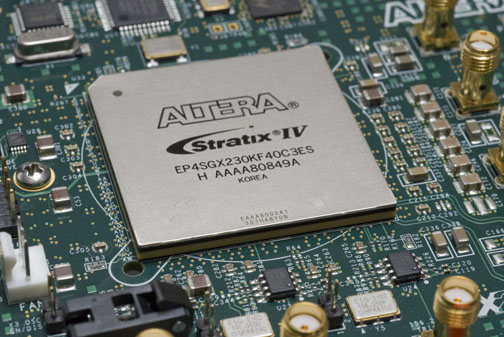
\includegraphics[width=0.48\textwidth]{sample_1.jpg}
    \caption{Diagrama o resultado del Ejercicio 1}
    \label{fig:ejercicio1}
\end{wrapfigure}

En este ejercicio se desarrolla [descripción del ejercicio]. A continuación se presenta el análisis y la implementación realizada.

Como se puede observar en la Figura \ref{fig:ejercicio1}, [explicación de la imagen]. Este ejercicio requiere una comprensión profunda de los conceptos
fundamentales estudiados en clase, así como la capacidad de aplicarlos en situaciones prácticas.

El desarrollo de este ejercicio implica varios pasos importantes que deben seguirse cuidadosamente. Primero, es necesario analizar el problema planteado
y comprender todos sus requisitos. Luego, se debe diseñar una solución apropiada que cumpla con todos los criterios especificados.

\subsection{Ejercicio 2}

Para el segundo ejercicio, se implementó [descripción del ejercicio]. El proceso seguido fue el siguiente:

\begin{enumerate}
    \item Análisis del problema
    \item Diseño de la solución
    \item Implementación del código
    \item Pruebas y validación
\end{enumerate}

\begin{figure}[H]
    \centering
    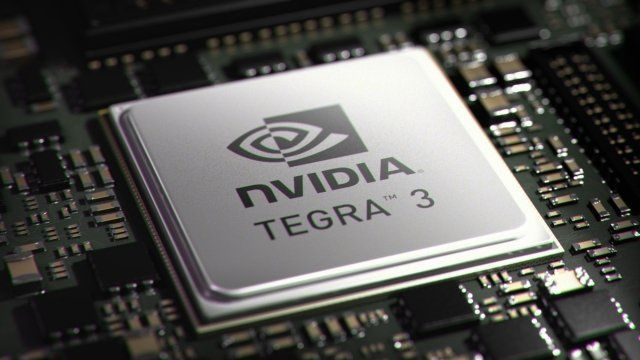
\includegraphics[width=0.65\textwidth]{sample_2.jpeg}
    \caption{Captura de pantalla o diagrama del Ejercicio 2}
    \label{fig:ejercicio2}
\end{figure}

La Figura \ref{fig:ejercicio2} muestra [explicación de la imagen].

\subsection{Ejercicio 3}

\begin{wrapfigure}{l}{0.45\textwidth}
    \centering
    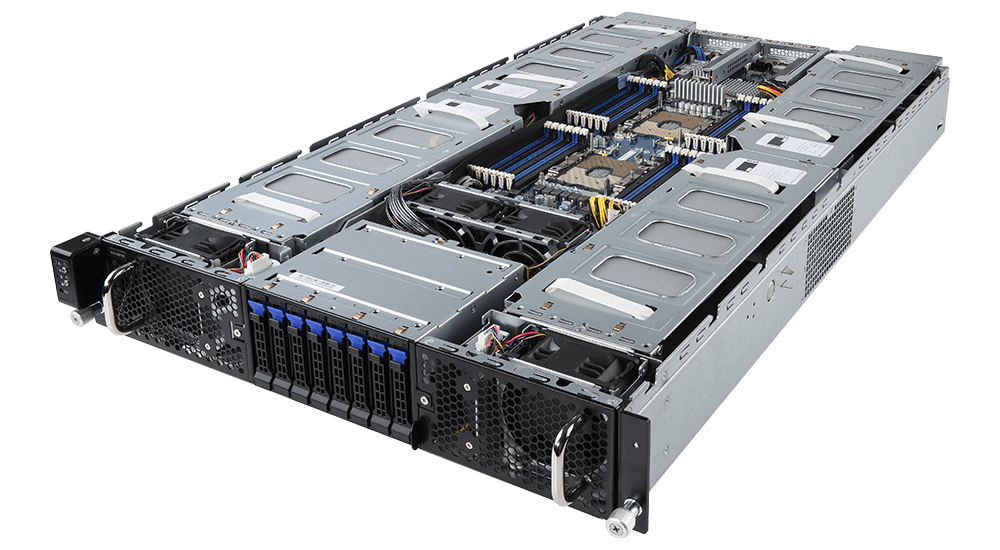
\includegraphics[width=0.43\textwidth]{sample_3.jpg}
    \caption{Resultados del Ejercicio 3}
    \label{fig:ejercicio3}
\end{wrapfigure}

El tercer ejercicio presenta un desafío adicional respecto a los anteriores, ya que combina varios conceptos estudiados. La implementación debe ser
eficiente y cumplir con los requisitos de rendimiento establecidos.

Como muestra la Figura \ref{fig:ejercicio3}, los resultados obtenidos demuestran la correcta aplicación de las técnicas aprendidas. Es importante destacar
que la solución implementada no solo resuelve el problema planteado, sino que también optimiza el uso de recursos del sistema.

La metodología seguida para resolver este ejercicio incluye pruebas exhaustivas y validación de resultados en diferentes escenarios.

\section{Código Fuente}

A continuación se presenta el código implementado para los ejercicios:

\subsection{Código del Ejercicio 1}

\begin{lstlisting}[caption={Implementación del Ejercicio 1}, label={lst:ejercicio1}]
#include <stdio.h>
#include <stdlib.h>

int main() {
    // Código de ejemplo - reemplazar con tu implementación
    printf("Ejercicio 1: Hola Mundo\n");
    
    // Tu código aquí
    
    return 0;
}
\end{lstlisting}

\subsection{Código del Ejercicio 2}

\begin{lstlisting}[caption={Implementación del Ejercicio 2}, label={lst:ejercicio2}]
#include <stdio.h>
#include <stdlib.h>

int main() {
    // Código de ejemplo - reemplazar con tu implementación
    printf("Ejercicio 2\n");
    
    // Tu código aquí
    
    return 0;
}
\end{lstlisting}

\section{Resultados}

En esta sección se analizan los resultados obtenidos durante la ejecución de los ejercicios.

\subsection{Resultados del Ejercicio 1}

\begin{figure}[H]
    \centering
    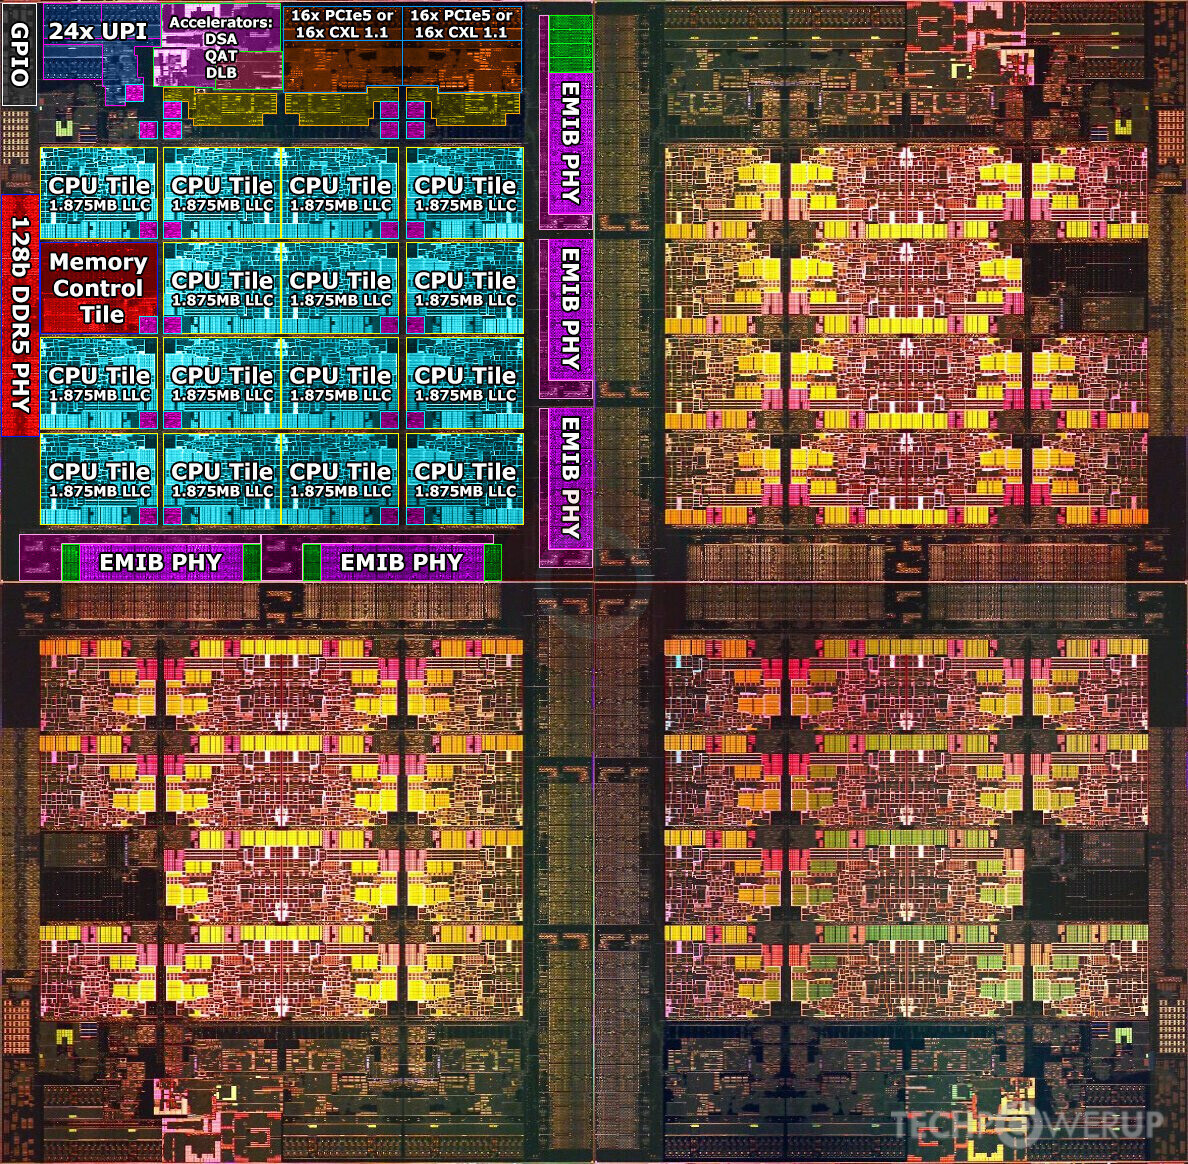
\includegraphics[width=0.7\textwidth]{sample_4.jpg}
    \caption{Resultados de la ejecución del Ejercicio 1}
    \label{fig:resultados1}
\end{figure}

Los resultados mostrados en la Figura \ref{fig:resultados1} indican que [análisis de resultados].

\subsection{Resultados del Ejercicio 2}

\begin{figure}[H]
    \centering
    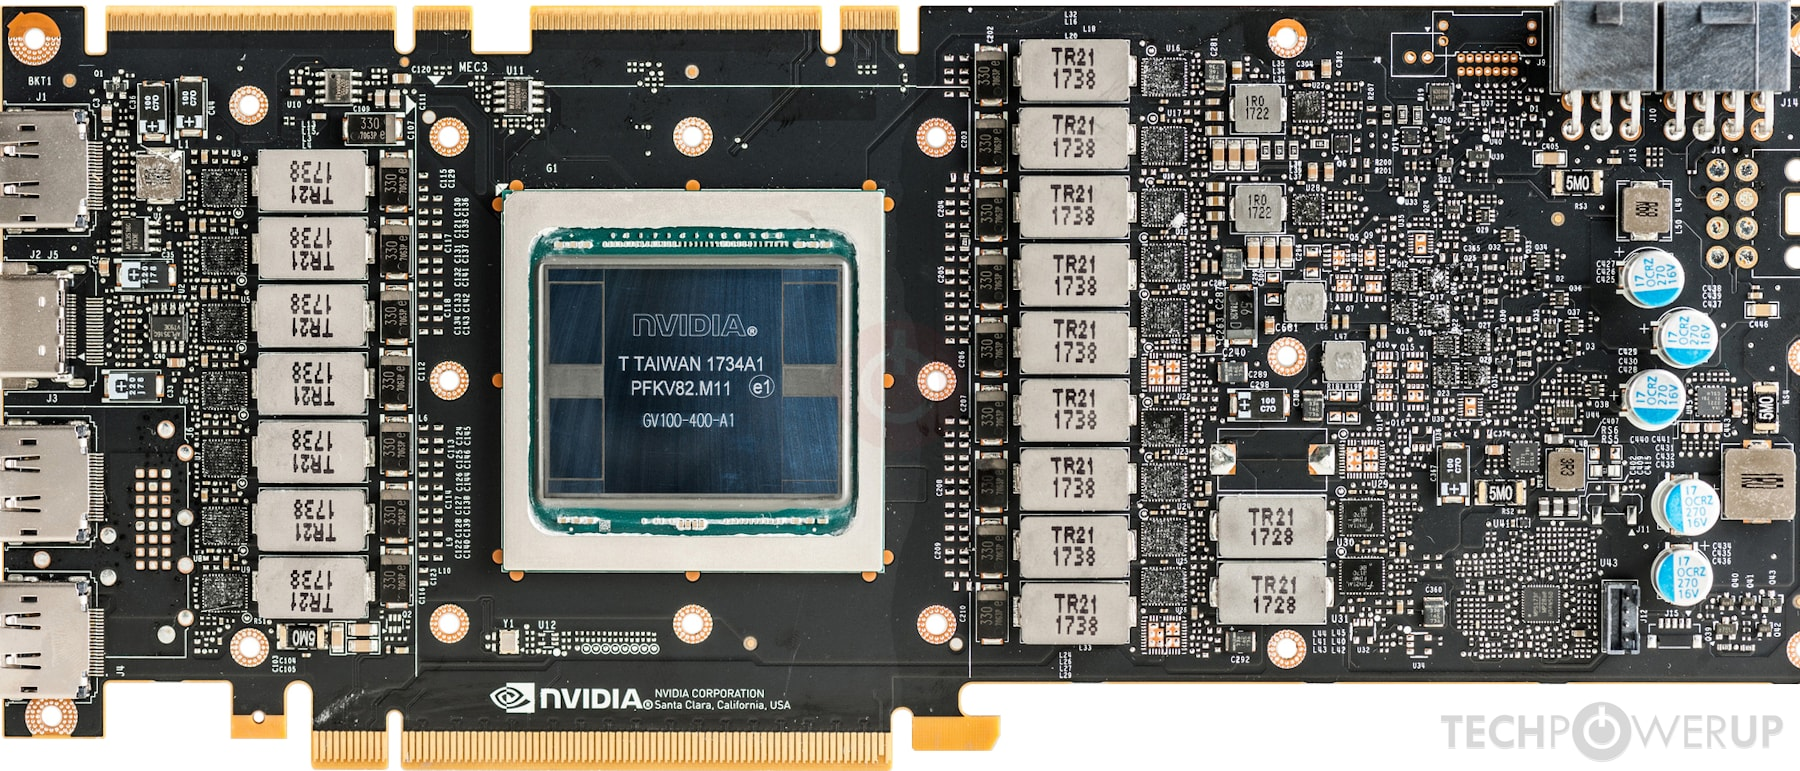
\includegraphics[width=0.7\textwidth]{sample_5.jpg}
    \caption{Resultados de la ejecución del Ejercicio 2}
    \label{fig:resultados2}
\end{figure}

Según se observa en la Figura \ref{fig:resultados2}, [análisis de resultados].

\subsection{Comparativa de Resultados}

\begin{wrapfigure}{r}{0.5\textwidth}
    \centering
    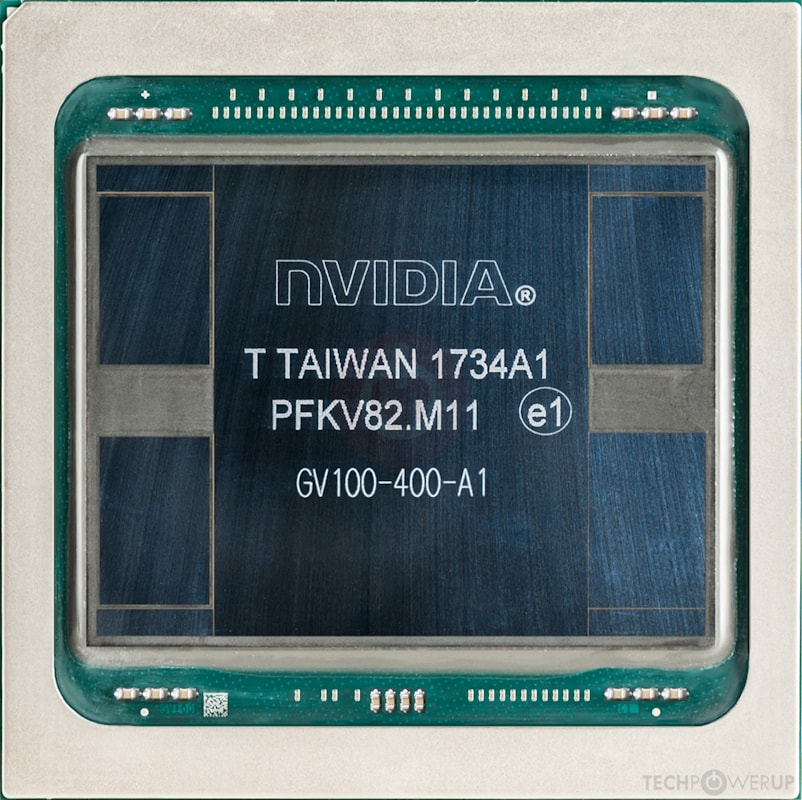
\includegraphics[width=0.48\textwidth]{sample_6.jpg}
    \caption{Comparativa de rendimiento entre ejercicios}
    \label{fig:comparativa}
\end{wrapfigure}

La comparativa presentada en la Figura \ref{fig:comparativa} permite visualizar las diferencias de rendimiento entre los distintos ejercicios implementados.
Los datos recopilados muestran patrones interesantes que merecen un análisis detallado.

Se puede observar que cada ejercicio presenta características particulares en cuanto a tiempo de ejecución, uso de memoria y eficiencia general. Estos 
resultados son coherentes con las expectativas teóricas y confirman la validez de las implementaciones realizadas.

El análisis comparativo revela áreas de mejora potenciales y confirma las decisiones de diseño tomadas durante el desarrollo de cada ejercicio.

\clearpage

\section{Conclusiones}

Tras la realización de esta práctica, se pueden extraer las siguientes conclusiones:

\begin{itemize}
    \item Conclusión 1
    \item Conclusión 2
    \item Conclusión 3
\end{itemize}

\begin{figure}[H]
    \centering
    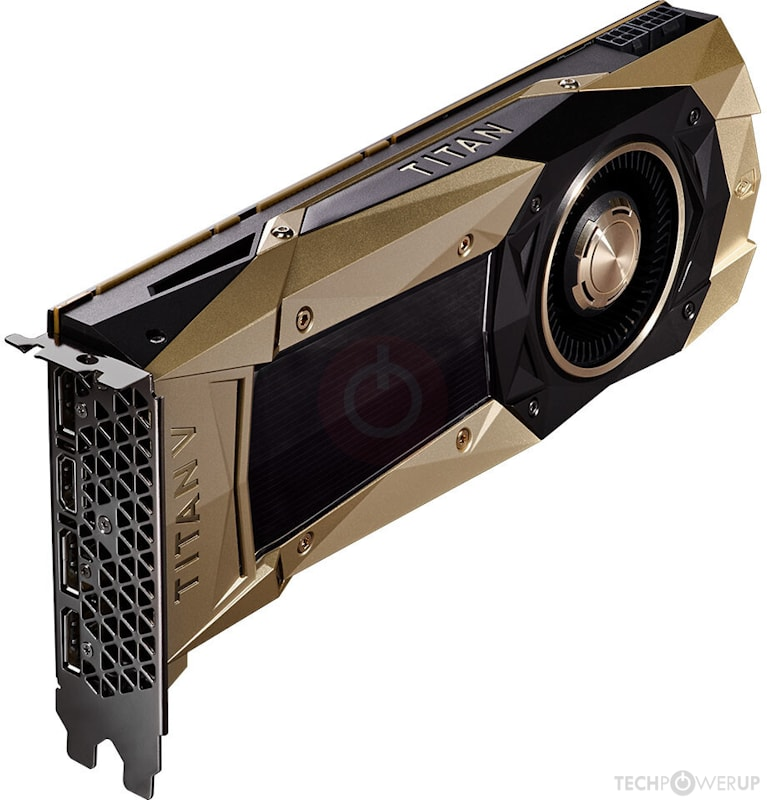
\includegraphics[width=0.6\textwidth]{sample_7.jpg}
    \caption{Diagrama resumen o conclusión final}
    \label{fig:conclusion}
\end{figure}

Como se resume en la Figura \ref{fig:conclusion}, [conclusión final].

\section{Bibliografía}

\begin{itemize}
  \item Referencia 1: [Autor]. [Título]. [Editorial], [Año].
  \item Referencia 2: [Autor]. [Título]. [Editorial], [Año].
  \item Documentación oficial de [herramienta/lenguaje utilizado]
\end{itemize}
  
\end{document}